\documentclass[conference]{IEEEtran}

\usepackage{listings}
\usepackage{pgfplots}
\pgfplotsset{compat=1.6}
\usepackage{hyperref}
\usepackage{caption}
\usepackage{subcaption}
\usepackage{tikz}

\usepackage[
  backend=biber,
  style=ieee,
  sorting=none
]{biblatex}
\addbibresource{CAD.bib}

\lstset{basicstyle=\footnotesize\ttfamily,
  breaklines=true}

\begin{document}

\title{Performance enhancement using MPI in a simulation of heat diffusion}

\author{
  \IEEEauthorblockN{Gonçalo Lourenço \\ nº55780 \\ gm.lourenco@campus.fct.unl.pt}
  \and
  \IEEEauthorblockN{Joana Faria \\ nº55754 \\ js.faria@campus.fct.unl.pt}
}

\maketitle



\section{Introduction}
This assignment aims to optimize a base code, written in \texttt{C}, that computes a simulation for heat diffusion. This time we intend to parallelize the computation using the Message Passing Interface (MPI).

To find the best performance we will explore different approaches, namely analyzing different patterns of communication and trying to overlap the communication with the computation.

We have available, for this assignment, two nodes, each one with 16 true CPUs.\@ Given this information, we can have a maximum of 32 processes.


\section{Results}
We experiment with several versions of a parallel program using MPI, these versions are explained and analyzed below.

To establish a baseline for comparison we start by analyzing the execution time of the sequential version and we obtain an average of 153.99 seconds, with the following parameters:
\begin{verbatim}
  // Width of the area
  const int nx = 200;
  // Height of the area
  const int ny = 200;
  // Diffusion constant           
  const float a = 0.5;
  // h=dx=dy  grid spacing
  const float h = 0.005;
  // Number of time steps to simulate
  const int numSteps = 100000;  
  // How frequently to write output image
  const int outputEvery = 100000;
\end{verbatim}

Unless otherwise stated, these will be the parameters used for determining the execution times. The average execution time was calculated using 10 executions.

\subsection{V1 version --- Synchronous Communication}\label{sec:v1}

In version V1 we start with a simple parallel version where we distribute the lines of the original matrix by the number of processes and perform synchronous communication between neighbors processes to obtain the border necessary for the computation.

For the communication necessary to write the output we use the \texttt{MPI\_Send} and \texttt{MPI\_Recv} methods, where all process sends their results to process 0, which aggregates all the results and writes the output file.

In \autoref{fig:executionTimeV1} we can see the execution time for V1, comparing the performance of this version for different numbers of processes. From this graphic we can see the bigger improvement until 16 processes, these processes run on the same machine. For the sake of completeness, we test with 17 processes and we can observe a slight worsening, this is because only one process is running on a different machine, adding communication overhead. Is due to this communication overhead that the improvements aren't bigger when we use 32 or 48 processes.

\begin{figure}[ht]
  \centering
  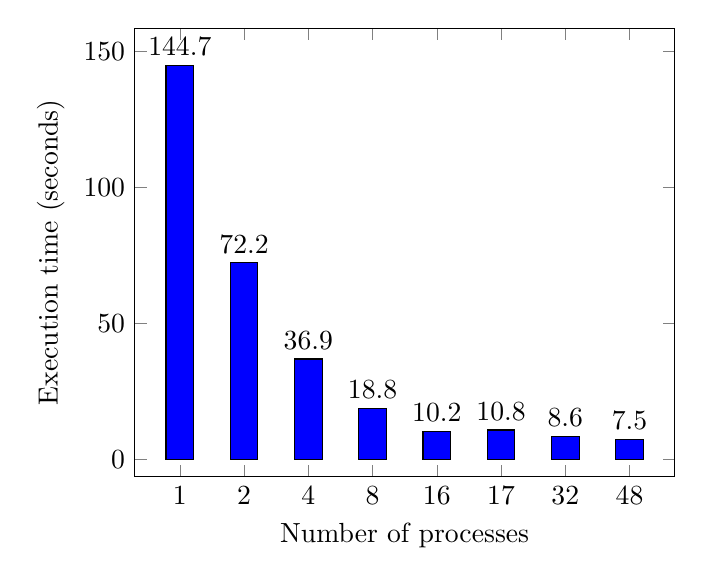
\begin{tikzpicture}

    \begin{axis}[
        ylabel={Execution time (seconds)},
        xlabel={Number of processes},
        symbolic x coords={1,2, 4, 8, 16, 17, 32, 48},
        xtick=data,
        nodes near coords={
            \pgfmathprintnumber[precision=1]{\pgfplotspointmeta}
          },
      ]
      \addplot[ybar,fill=blue] coordinates {
          (1,   144.74)
          (2,   72.22)
          (4,  36.92)
          (8,   18.83)
          (16,   10.23)
          (17,   10.83)
          (32,   8.57)
          (48,   7.45)
        };
    \end{axis}
  \end{tikzpicture}
  \caption{Execution time of V1 varying the number of processes}
  \label{fig:executionTimeV1}
\end{figure}

\subsection{V2 --- Gather}\label{sec:v2}
In this version, we modify version V1 to use the method \texttt{MPI\_Gather} instead of the \texttt{MPI\_Send} and \texttt{MPI\_Recv} methods for communication for the phase of writing the output. The results are presented in \autoref{fig:executionTimeV2}.

The results we obtain are essentially the same, which is to be expected since both V1 and V2 do the same thing. With this version, we intended to discover if the method had some level of extra optimization but we found none.

We also considered the use of the method \texttt{MPI\_Allgather} but it wouldn't be a wise choice due to the lack of use for the data we transferred to the other nodes would have.

\begin{figure}[ht]
  \centering
  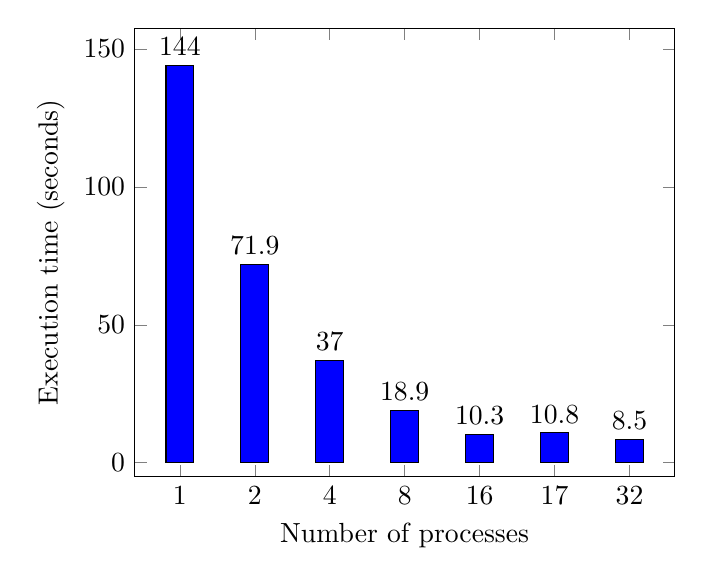
\begin{tikzpicture}

    \begin{axis}[
        ylabel={Execution time (seconds)},
        xlabel={Number of processes},
        symbolic x coords={1,2, 4, 8, 16, 17, 32},
        xtick=data,
        nodes near coords={
            \pgfmathprintnumber[precision=1]{\pgfplotspointmeta}
          },
      ]
      \addplot[ybar,fill=blue] coordinates {
          (1,   144)
          (2,   71.88)
          (4,  37.03)
          (8,   18.91)
          (16,   10.26)
          (17,   10.80)
          (32,   8.51)
        };
    \end{axis}
  \end{tikzpicture}
  \caption{Execution time of V2 varying the number of processes}
  \label{fig:executionTimeV2}
\end{figure}

\subsection{V3 --- One node for output}
In V3 we assign node 0 the function of joining the output of all the other nodes, performing no computation concerning the heat equation. This version was intended as a first step to overlap computation with communication in situations where output is stored more frequently. In V3, we also kept the communication synchronous.

The average execution time we obtained for this version was 8.52 seconds.

\subsection{V4 --- Assyncronous communication}
V4 was built using V3 as a base but with the use of asynchronous communication in the steps for writing the output. Node 0 receives, asynchronously, from every other node the result of their computation, after which it will process it as output so that the other nodes can immediately start the computation of the next step of the heat equation.

This version had an average execution time of 8.52 seconds.


\section{Discussion}

All our results are gathered in the \texttt{results} folder and aggregated in the file \texttt{results/results.xlsx}.

Now we want to compare the results of our different versions. In \autoref{fig:executionTimeOneOutput} we can see the comparison of our version while running with 32 processes and only one output at the end of all iterations. As we can see there aren't any performance differences, this is expected since the main advantage of V4 is the possibility of overlap computation with communication. With only one output this advantage isn't explored so we obtain the same performance.

\begin{figure}[ht]
  \centering
  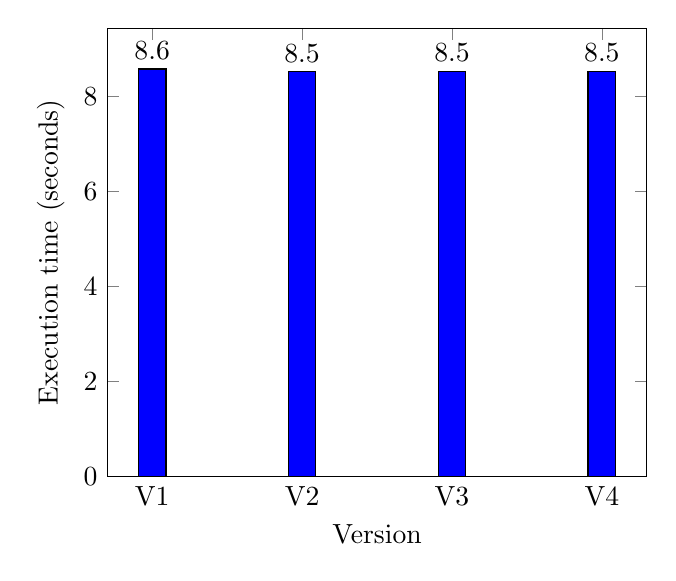
\begin{tikzpicture}

    \begin{axis}[
        ylabel={Execution time (seconds)},
        xlabel={Version},
        ymin = 0,
        symbolic x coords={V1, V2, V3, V4},
        xtick=data,
        nodes near coords={
            \pgfmathprintnumber[precision=1]{\pgfplotspointmeta}
          },
      ]
      \addplot[ybar,fill=blue] coordinates {
          (V1,   8.57)
          (V2,   8.51)
          (V3,  8.52)
          (V4,   8.52)
        };
    \end{axis}
  \end{tikzpicture}
  \caption{Comparison of different versions with \texttt{outputEvery = 100000} and 32 processes}
  \label{fig:executionTimeOneOutput}
\end{figure}

To explore all the potential of overlapping communication with computation we test our version with
\texttt{outputEvery = 100} and the results are presented in \autoref{fig:executionTimeManyOutputs}.
We can conclude that having one node solely responsible for producing the output allows much better performance than the versions where the node gathering the output also does computation for the heat equation.

\begin{figure}[ht]
  \centering
  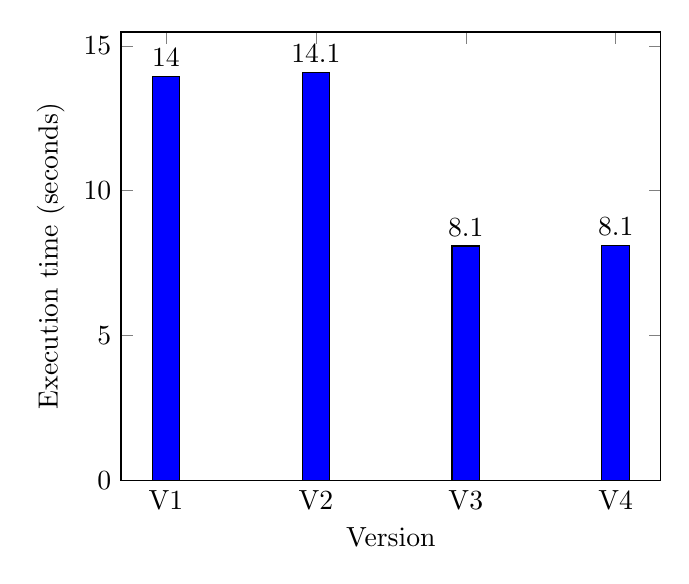
\begin{tikzpicture}

    \begin{axis}[
        ylabel={Execution time (seconds)},
        xlabel={Version},
        ymin = 0,
        symbolic x coords={V1, V2, V3, V4},
        xtick=data,
        nodes near coords={
            \pgfmathprintnumber[precision=1]{\pgfplotspointmeta}
          },
      ]
      \addplot[ybar,fill=blue] coordinates {
          (V1,   13.95)
          (V2,   14.07)
          (V3,  8.09)
          (V4,   8.12)
        };
    \end{axis}
  \end{tikzpicture}
  \caption{Comparison of different versions with \texttt{outputEvery = 100} and 32 processes}
  \label{fig:executionTimeManyOutputs}
\end{figure}

Contrary to expectations V3 and V4 showed the same performance. This may be due to the fact that one node responsible for the output allows enough overlap of the output writing with the next computation.

We left the communication between neighbor processes synchronous because it makes little to no sense to do it asynchronously since the processes need the data sent to the next computation and it's not possible to proceed without this data.

Comparing all these parallel versions with the sequential version we can see the impact of parallelization. We were able to go from 153.99 seconds of execution time with the version to 10.23 seconds using only one machine and 16 processes, with room to scale up.

Despite the same result as V3, we select V4 as our best version for this project.

It may be important to refer that the same problem was solved in one-fourth of the time using the GPU for the same calculations while reserving the CPU only for output. This makes the solution we obtained for our last project better, but, it has the restriction of needing a GPU (a dedicated NVIDIA GPU in this case) while the MPI solution is already a big improvement (15x) from the sequential solution using only CPU cores which are more accessible.

\section{Compilation and Execution Instructions}
Our best version, V4, can be compiled and executed with the following commands, executed from inside the folder \texttt{./proj2}:
\begin{verbatim}
mpicc -o v4 v4.c -lm

oarsub -l nodes=2
'mpirun --mca btl_tcp_if_include bond0
--hostfile $OAR_NODEFILE v4 y'
\end{verbatim}

The execution command has to be executed from the frontend of the DI Cluster and the execution will be across to machines in a total of 32 processes. The execution will output every 100 steps and the result will be saved in folder \texttt{./images/V4}.

All the code is available in the \texttt{./proj2} folder.


\end{document}